\documentclass[12pt,a4,oneside,usenames,dvipsnames]{book}
  \usepackage{polyglossia}
  \usepackage{fontspec}
  \setmainlanguage{english}
  \setotherlanguage{greek}
  \setmainfont[Scale=1.00]{Junicode}
  \usepackage{unicode-math}
  %\setmathfont{Latin Modern Math}
  \setmathfont{TeX Gyre Pagella Math}
  \usepackage{microtype}
  \usepackage{dot2texi}
  \usepackage{hyperref}
\hypersetup{
    unicode,
    verbose=false,
    pdfpagelayout=TwoColumnRight,
    bookmarksopen,
    colorlinks,
    citecolor=black,
    filecolor=black,
    linkcolor=black,
    urlcolor=black
}
  \usepackage{microtype}
  \usepackage{amsmath}
  \usepackage{float}
  \usepackage{skeldoc}
  \floatplacement{figure}{H}
  \usepackage{tikz}
  \usepackage{svg}
  \usepackage{metalogo}
  \usepackage{csquotes}
  \usepackage[compact,nostruts,medium]{titlesec}
  %\titlespacing*{\chapter}{0pt}{0pt}{0pt}
  \newcommand\makeskelfig{%
  \begin{figure}
  {\centering%
  \skelfig[width=0.4\textwidth]{2\baselineskip}%
  \skelcaption[width=0.2\textwidth,lines=1]{}}
  \end{figure}}
  \usepackage{setspace}
  \usepackage{xcolor}
  \definecolor{bgcolor}{rgb}{0.95,0.95,0.95}
  \definecolor{red}{rgb}{1,0,0}
  \definecolor{gray}{RGB}{24,24,24}
   \definecolor{thered}    {rgb} {0.65,0.04,0.07}
 \definecolor{thegreen}  {rgb} {0.06,0.44,0.08}
 \definecolor{theblue}   {rgb} {0.02,0.04,0.48}
 \definecolor{sectioning}{gray}{0.44}
 \definecolor{thegrey}   {gray}{0.5}
 \definecolor{theframe}  {gray}{0.75}
 \definecolor{theshade}  {gray}{0.94}
\usepackage[cache=false,outputdir=build]{minted}
\setminted[tex]{breaklines=true,linenos=true,bgcolor=theshade,frame=single,framesep=5pt,rulecolor=theframe}
\setminted[shell]{breaklines=true,linenos=true,bgcolor=theshade,frame=single,framesep=5pt,rulecolor=theframe}
\definecolor{bg}{rgb}{0.95,0.95,0.95}
\usepackage{xspace}
\usepackage{contour}
\usepackage[normalem]{ulem}

\renewcommand{\ULdepth}{1.8pt}
\contourlength{0.8pt}

\newcommand\colorunderline[1]{\bgroup\markoverwith{\textcolor{#1}{\rule[-0.5ex]{2pt}{0.8pt}}}\ULon}
\newcommand{\myuline}[2]{%
  \colorunderline{#1}{\phantom{#2}}%
  \llap{\contour{white}{#2}}%
}
\newcommand{\myurl}[2]{%
  \href{#1}{\myuline{blue}{#2}}%
}

\newcommand\titletext{Anatomy of \enquote{Anatomy of Melancholy} in \XeLaTeX{}}
\title{\titletext{}}
\newcommand\subtitle{\emph{Making a \emph{large} and \emph{complex} book with \emph{free/libre}~software}}
\newcommand\biblatex{\texttt{biblatex}\xspace}%
\hypersetup{
  pdftitle={\titletext{}},
  pdfauthor={epilys},
  pdfsubject={programming},
}
\begin{document}
\setstretch{1.1}
\addtolength{\parskip}{5pt}%
\newlength\drop
\thispagestyle{empty}
\begingroup% Harry Carter
\setlength{\drop}{0.1\textheight}
\vspace*{\drop}
\begin{flushleft}
    \rule{\textwidth}{1.6pt}%
    \vspace{-0.9\baselineskip}
    \rule{\textwidth}{0.4pt}\\[0.8\baselineskip]
    {\centering
    \scalebox{2.0}{\parbox{0.5\textwidth}{\centering\Huge{}\textsc{{\titletext{}}}}}\\
    \vspace{1.5\baselineskip}
    {\LARGE\subtitle{}}\par
    \vspace*{0.3\baselineskip}
    }\rule{\textwidth}{1.6pt}%
    \vspace{-0.9\baselineskip}
    \rule{\textwidth}{0.4pt}\\[0.5\baselineskip]
    {\Large{}epilys}\hfill{\small{}\today{}}
\vfill%
\end{flushleft}%
\endgroup
\clearpage{}
\tableofcontents
\part{Introduction}
\chapter{Selecting a typeface (Junicode)}
\skelpars{3}

\chapter{Selecting a paper layout and margins}
\skelpar
%
\begin{figure}{\centering%
\skelfig[width=0.4\textwidth]{2\baselineskip}%
\skelcaption[width=0.2\textwidth,lines=1]{}}
\end{figure}{}
\skelpar
%
\begin{figure}{\centering%
\skelfig[width=0.4\textwidth]{2\baselineskip}%
\skelcaption[width=0.2\textwidth,lines=1]{}}
\end{figure}{}
\skelpars{2}

\chapter{Selecting a design style, choices}
\skelpars{3}

\chapter{Organizing the artwork with \biblatex\label{ch:biblatex}}

To simplify the handling of a large amount of artwork in the book, we store each work as a bibliography entry in a \texttt{bib} database and use the bibliography management package \myurl{https://ctan.org/pkg/biblatex?lang=en}{biblatex}. The \texttt{bib} database is a plain text file with entries of the following format:

\begin{minted}{tex}
@Misc{TheLoveSong,
  title        = {The Love Song},
  annotation   = {{Burne-Jones associated this painting with a refrain from a French folk ballad: "Alas, I know a love song, / Sad or happy, each in turn." Cupid, his arrows slung over his shoulder, works the bellows on the portative organ. This picture, which took nine years to complete, unites inspirations that shaped Burne-Jones’s art: medievalism, Italian Renaissance painting, romance, beauty, and music. Like a bittersweet melody, the scene suggests a mood of dreamy melancholy. As one critic observed, "There is no story: nothing to guess at, but everything to feel."}},
  author       = {{Edward Burne-Jones}},
  date         = {1868/1877},
  url          = {https://www.metmuseum.org/art/collection/search/435826},
  note         = {47.26},
  file         = {The-Love-Song-Edward-Burne-Jones-small.jpg},
  type         = {oil on canvas},
  keywords     = {artwork},
}
\end{minted}

We use the \texttt{file} field to store the image filename. Assuming the images are stored in a folder called \texttt{figures} in the same directory as the main \TeX\ file, we define the default graphics path as

\begin{minted}{tex}
\graphicspath{{./figures/}}
\end{minted}

This means that everytime we include a graphic with the \texttt{includegraphics} macro, it will look for it in that prepend the path to whatever we pass to \texttt{includegraphics}.

To load the database we insert this line in our main \texttt{tex} file:

\begin{minted}{tex}
\addbibresource{citations.bib}
\end{minted}

Now, using the key for each entry we can use any of the entry fields inside the document. The fields we are interested in are:

\begin{itemize}
  \item \texttt{author}
  \item \texttt{title}
  \item \texttt{year}
  \item \texttt{type}, which contains the art medium
  \item \texttt{file}
\end{itemize}

\biblatex defines macros to access the fields using the entry key.

\skelpar
%
\begin{figure}{\centering%
\skelfig[width=0.4\textwidth]{2\baselineskip}%
\skelcaption[width=0.2\textwidth,lines=1]{}}
\end{figure}{}
\skelpars{2}

\part{Premilinary pages}

\chapter{Designing a cover with Inkscape}
%
\begin{figure}{\centering%
\skelfig[width=0.4\textwidth]{2\baselineskip}%
\skelcaption[width=0.2\textwidth,lines=1]{}}
\end{figure}{}
\skelpars{2}
%
\begin{figure}{\centering%
\skelfig[width=0.4\textwidth]{2\baselineskip}%
\skelcaption[width=0.2\textwidth,lines=1]{}}
\end{figure}{}

\chapter{Designing a diagram for the frontispiece with \texttt{TiKz}}
%
\begin{figure}{\centering%
\skelfig[width=0.4\textwidth]{2\baselineskip}%
\skelcaption[width=0.2\textwidth,lines=1]{}}
\end{figure}{}
\skelpars{2}

\chapter{Including the cover, title pages and frontispiece}
\skelpars{2}

\chapter{Adding a list of figures and a list of prescriptions}
%
\begin{figure}{\centering%
\skelfig[width=0.4\textwidth]{2\baselineskip}%
\skelcaption[width=0.2\textwidth,lines=1]{}}
\end{figure}{}
\skelpars{2}

\part{Main Part}

\chapter{Creating formatting and helpful macros}
\skelpars{3}

\section{\textsc{URL}s}

Underlined text is not considered particularly pleasing. However, it's an established visual hint for hyperlinks, and we will use it for linking to the book's \texttt{git} repository and the typeface websites.

Using the \myurl{https://ctan.org/pkg/contour}{contour} package, we can draw the outline of each glyph behind the glyph itself. That way, the descenders of a glyph, which is the part of the glyph going bellow the base line, do not cross the underline:
\vspace{\baselineskip}
\begin{figure}{\centering%
\scalebox{4.0}{\mbox{\myurl{www.example.com}{hyperlink,}}}\par
  }
\end{figure}

\begin{minted}{tex}
\usepackage{contour}
\usepackage[normalem]{ulem}

\renewcommand{\ULdepth}{1.8pt}
\contourlength{0.8pt}

\newcommand\colorunderline[1]{\bgroup%
  \markoverwith{%
    \textcolor{#1}{%
      \rule[-0.5ex]{2pt}{0.8pt}%
    }%
  }%
  \ULon%
}
\newcommand{\myuline}[2]{%
  \colorunderline{#1}{\phantom{#2}}%
  \llap{\contour{white}{#2}}%
}
\newcommand{\myurl}[2]{%
  \href{#1}{\myuline{blue}{#2}}%
}
\end{minted}

\chapter{Converting the end notes to a usable format}
\skelpars{3}

\chapter{Using footnotes or margin notes}
\skelpars{3}

\chapter{Typesetting figures}\label{ch:figures}
\skelpar

\section{Placing figures in the text}
\skelpar

\section{Placing figures on their own page}
\skelpar

\chapter{Designing the synopsis schemata}
\skelpars{3}

\chapter{Typesetting the author's notes}
\skelpars{3}

\chapter{Typesetting inline translations}
\skelpars{3}

\chapter{Finding out uncommon vocabulary for a glossary}
\skelpars{3}

\chapter{Typesetting verse and block quotations}
\skelpars{3}

\chapter{Creating an \texttt{OTF} for Chaucer with FontForge}
\skelpars{3}

\part{Appendices}

\chapter{Creating an index for author and topic references}
\skelpars{3}

\chapter{Designing a custom \biblatex bibliography style to list artwork sources}

\begin{figure}
  \centering
  \qquad\begin{minipage}{0.3\textwidth}%
    \frame{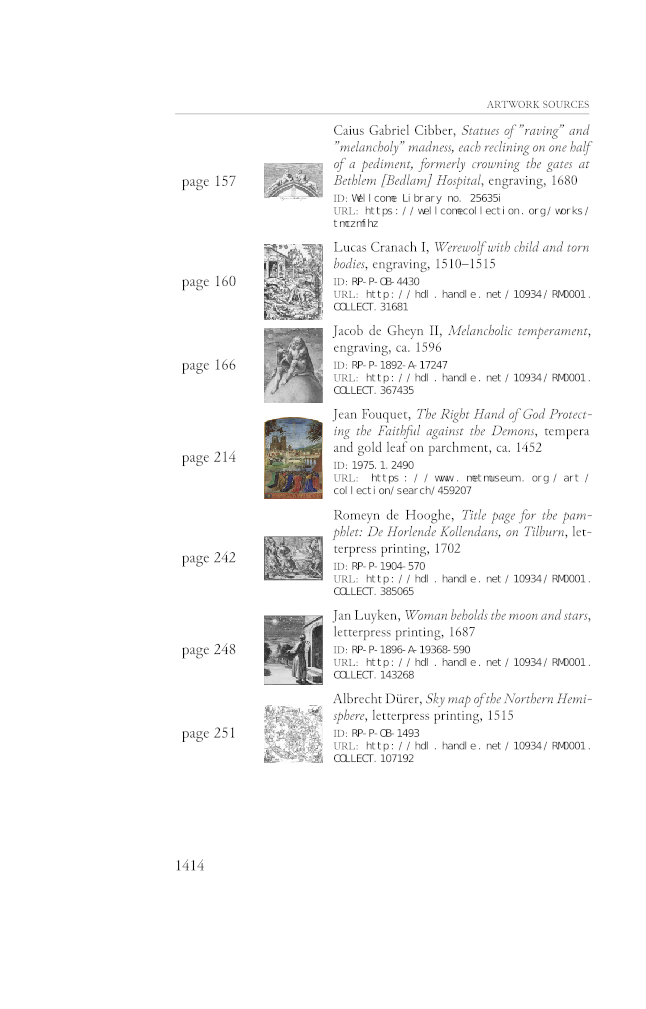
\includegraphics[keepaspectratio,height=60mm, width=100mm]{aoaom/artbiblverso.png}}
  \end{minipage}%
  \quad\begin{minipage}{0.3\textwidth}%
    \frame{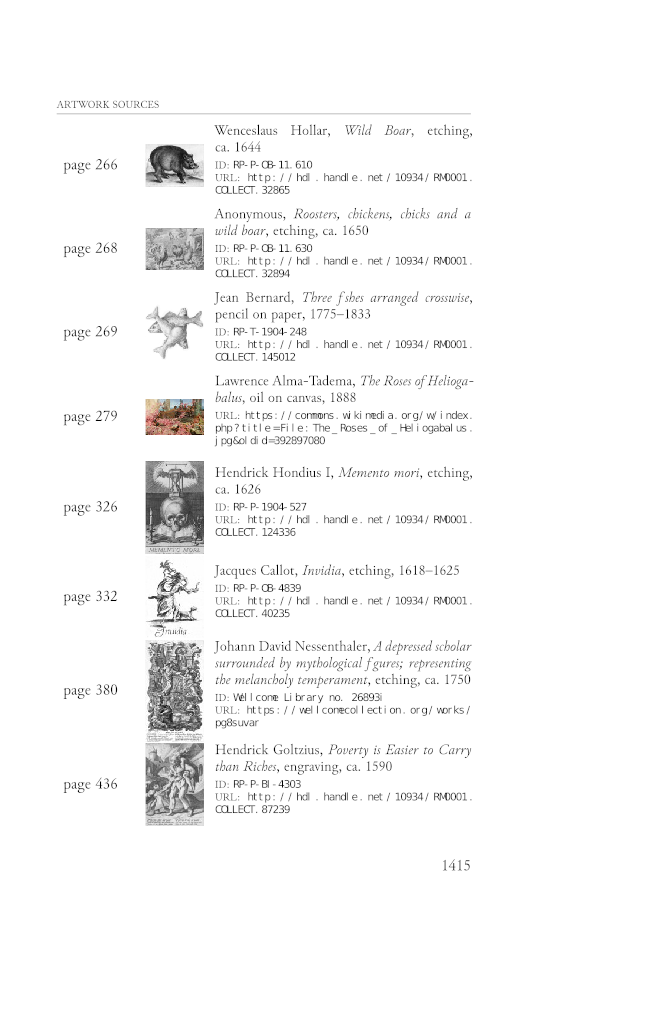
\includegraphics[keepaspectratio,height=60mm, width=100mm]{aoaom/artbiblrecto.png}}
  \end{minipage}%
  \caption{\footnotesize{}Pagespread of art bibliography.}
\end{figure}

We want to add a list of the artworks included in the book and their
sources. We saw how the artwork database was compiled in a \texttt{bib}
file back in chapter \hyperref[ch:biblatex]{\ref{ch:biblatex}}.

\biblatex prints the bibliography with a
\texttt{\textbackslash{}printbibliography} macro. The invocation used in
the book is:

\begin{minted}{tex}
\defbibnote{introduction}{All artworks are in the public domain.}
\phantomsection
\printbibliography[label=app:artworksources,
                   prenote=introduction,
                   heading=bibnumbered,
                   title={Artwork Sources}]
\end{minted}

This will print a chapter with title \texttt{Artwork Sources} and a paragraph
after the title, set with the \texttt{prenote} option and defined with a
preceding \texttt{defbibnote} command.

Using the \texttt{numeric} bibliography style, the result is this:

\begin{figure}
{\centering%
\skelfig[width=0.4\textwidth]{2\baselineskip}%
\skelcaption[width=0.2\textwidth,lines=1]{}}
\end{figure}

Let's copy the numeric source file, called \texttt{numeric.bbx} to the
project's folder and name it \texttt{art-numeric.bbx}.

We want to show a list of every artwork with its name, title,
format/medium, year, the source URL and the source's identification
number (called \emph{accession number} by librarians). For extra
fanciness, let's show a thumbnail of the work and the page where it's
located.

First, we want instead of index label numbering to show the page
location of each artwork. This is done by defining the bibliography's
environment with
\texttt{\textbackslash{}defbibenvironment\{bibliography\}}:

\begin{figure}
{\centering%
\skelfig[width=0.4\textwidth]{2\baselineskip}%
\skelcaption[width=0.2\textwidth,lines=1]{}}
\end{figure}

We want every label to have the same width, and a page number can range
from 1 to 3 digits for a book under 10\thinspace{}000 pages. So let's
set the label's width to the maximum width possible:

\begin{minted}{tex}
% This typesets the list entry labels for the artwork bibliography.
% The list is of this format:
%
% page X   [thumbnail] [details]
%
% page XY  [thumbnail] [details]
%
% page XYZ [thumbnail] [details]
%
% The "page XYZ" part is done in the following bibenvironment macro.
% We want the "page .." labels to have the same width regardless of
% how many digits the page is. For example we don't want a "Page 5"
% box to be smaller than a "Page 1234" box because this would cause
% misalignment of the list items.
%
% 1. Create new length to store the maximum page label width.
\newlength\PageRefLabelWidth
% 2. Create new box to store the maximum page label.
\newsavebox{\PageRefLabelBox}
% 3. Typeset a string that has the same width as the maximum page label
% (Book won't be more than 9999 pages, hopefully).
\savebox{\PageRefLabelBox}{\mbox{{page 9999}}}
% 4. Set length to width of box.
\setlength\PageRefLabelWidth{\wd\PageRefLabelBox}
\end{minted}

Then define the bibliography environment:

\begin{minted}{tex}
\defbibenvironment{bibliography}
  {\list
      % 5. and final step. put the page label in a box of set width.
     {\setlength{\fboxrule}{.5pt}\setlength{\fboxsep}{-.5pt}%
     \fbox{%
       \makebox[\PageRefLabelWidth]{%
         \usebibmacro{pagereflabel}%
      }}}%
     {\setlength{\labelwidth}{\PageRefLabelWidth}%
      \setlength{\leftmargin}{\labelwidth}%
      \setlength{\labelsep}{0pt}%
      \setlength{\itemsep}{\bibitemsep}%
      \setlength{\parsep}{\bibparsep}}%
      \renewcommand*{\makelabel}[1]{\hss##1}}
  {\endlist}
  {\item}
\endinput
\end{minted}

We have to decide on the layout of each
entry. Let's use the golden ratio $\phi$ which is a good bet.

The golden ratio which equals $\phi=1.618\ldots$, is two lengths $α$
and $β$ such that $α+β$ is to $α$ as $α$ is to $β$:

\begin{equation*}
\frac{α+β}{α}=\frac{α}{β}=\phi
\end{equation*}

We arbitrarily decide to set each thumbnail's maximum width to the width
of the string \enquote{\texttt{thumbnail:}}. Then, $β$ will contain
the page label and the thumbnail, and $α$ will contain the text with
the info.

\begin{figure}
  \centering
  \includesvg[keepaspectratio,height=60mm, width=100mm]{aoaom/artbib_a_b.svg}
\end{figure}

We last encountered length calculations in \autoref{ch:figures} where we calculated the space required for the annotation text of a figure. That required integer precision, and now we need floating point precision. To do the required arithmetic we use the
\mbox{\LaTeX$_{3_{\scriptstyle\varepsilon}}$} floating point interface
from the \myurl{https://ctan.org/pkg/xfp?lang=en}{xfp} package.

First, define $\phi$ as a length. $\phi$ is equal to
$\frac{\sqrt{5}+1}{2}$:

\begin{minted}{tex}
\edef\GoldenRatio{\fpeval{(sqrt(5)+1)/2}} % phi
\edef\GoldenRatioPlusOne{\fpeval{\GoldenRatio+1}} % phi+1
\end{minted}

Then $β=\phi\times{}α$ and $α=\frac{\text{\textbackslash{}textwidth}}{1+\phi{}}$:

\begin{minted}{tex}
\newlength\ArtInfoWidth
\newlength\ArtThumbnailWidth
\newlength\tmpAReg
\newlength\tmpBReg

\newsavebox{\TmpBoxForWidths}
\savebox{\TmpBoxForWidths}{\mbox{thumbnail:}}%
\setlength\ArtThumbnailWidth{\wd\TmpBoxForWidths}%

\setlength\tmpAReg{\fpeval{\textwidth/\GoldenRatioPlusOne}pt}
\setlength\ArtInfoWidth{\GoldenRatio\tmpAReg}
\setlength\tmpBReg{\tmpAReg-\PageRefLabelWidth-\ArtThumbnailWidth}
\end{minted}

Setting the thumbnail and the text in two \texttt{minipage}s we can put
them side by side:

\begin{figure}
{\centering%
\skelfig[width=0.4\textwidth]{2\baselineskip}%
\skelcaption[width=0.2\textwidth,lines=1]{}}
\end{figure}

To print the thumbnail let's define a custom \biblatex field
format. The file's relative path is stored in the \texttt{file} field of
each citation entry. We can define a custom format for printing the
\texttt{file} field:

\begin{minted}{tex}
\DeclareFieldFormat{includeartthumb}{{%
\graphicspath{{./figures/thumbs/}}%
\includegraphics[keepaspectratio,width=0.85\textwidth]{#1}}}
\end{minted}

This is a simple \texttt{\textbackslash{}includegraphics} \emph{only} it changes
\texttt{\textbackslash{}graphicspath} locally, that is inside the group
defined by the braces of the macro's definition. Recall that in
\autoref{ch:biblatex} we set \texttt{\textbackslash{}graphicspath} to
\texttt{./figures/}.

We create the thumbnails with a new \texttt{Makefile} target. First,
store the paths for each figure in a variable \texttt{\$INFILES} and the
thumb location, which will be inside \texttt{figures/thumbs}, in a
variable \texttt{\$OUTFILES}.

\begin{minted}{shell}
INFILES:=$(shell bash -c "grep file citations.bib| \
      cut -d '{' -f2 | cut -d'}' -f1 | sed 's/^/figures\//'")
OUTFILES:=$(shell bash -c "grep file citations.bib| \
      cut -d '{' -f2 | cut -d'}' -f1 | sed 's/^/figures\/thumbs\//'")
\end{minted}

Next, add the target dependency to the pdf:

\begin{minted}{shell}
anatomy-of-melancholy.pdf: main.tex *.tex $(OUTFILES)
\end{minted}

This means that before compiling the pdf, the targets
\texttt{figure/thumbs/foobar\_1}, etc. will have to be compiled first.
Let's add these targets:

\begin{minted}{shell}
figures/thumbs/%.jpg: figures/%.jpg
    @mkdir -p figures/thumbs
    convert -thumbnail 100 "$<" "$@"
\end{minted}

The first line creates the \texttt{thumbs} folder if it does not exist,
and the second is an \texttt{ImageMagick} command that makes a thumbnail
of width 100\texttt{px}.

Returning to \LaTeX, print the author, title, year, url, etc:

\begin{figure}
{\centering%
\skelfig[width=0.4\textwidth]{2\baselineskip}%
\skelcaption[width=0.2\textwidth,lines=1]{}}
\end{figure}

Observing the result in \autoref{fig:golden-ratio} we see that the
actual page dimensions end up as $\alpha+\beta=10.97\textrm{cm}$,
$\alpha=6.77\textrm{cm}$ and $\beta=4.20\textrm{cm}$. Indeed the
ratio checks out:\\
\begin{gather*}
\frac{\alpha+\beta}{\alpha}=\frac{10.97}{6.77}\approx{}1.6204\text{, and}\\
\frac{\alpha}{\beta}=\frac{6.77}{4.2}\approx{}1.612\text{ which is good enough.}
\end{gather*}

\begin{figure}
\centering
\includesvg[width=1\textwidth,height=\textheight]{aoaom/art-dims.svg}
\caption{Page layout and proportions\label{fig:golden-ratio}}
\end{figure}

\clearpage{}
\chapter{Adding an editor's postface}

\skelpars{3}
\chapter{Closing with a colophon}

\skelpars{3}
\end{document}
